In the previous chapter we restricted ourselves to observing various interesting locus-related phenomena in the confocal pair. 
Namely, we attempt to answer the following related questions:

\begin{itemize}
    \item When are loci algebraic?
    \item What is the type of curve for the locus of the incenter (and excenters) in a generic concentric, axis-parallel (CAP) pair?
    \item In \cite{sergei2016-com} it is shown that over Poncelet N-periodics in a generic pair of conics, the locus of vertex and area centroids is an ellipse. For triangles, both points collapse to $X_2$. Given 3-periodics in a generic pair of ellipses, when is the locus of some triangle center an ellipse? To answer we will use technique based on Blaschke products \cite{daepp-2019}, review below;
    \item We consider the special case of 3-periodics in a pair with a circumcircle, showing that many such loci are circles.
\end{itemize}

\section{When are Loci Algebraic?}
\label{sec:04-rational-trilinears}



Consider a Triangle Center $X$ whose Trilinears $p:q:r$ are rational on the sidelengths $s_1,s_2,s_3$, i.e., the Triangle Center Function $h$ is rational, see  
\cref{eqn:appAtrilin-cartesian}

\begin{theorem}
The locus of a rational triangle center
over 3-periodics in a CAP pair is an algebraic curve.
\label{thm:04-rational-center}
\end{theorem}

Our proof is based on the following 3-steps which yield an algebraic curve $\mathcal{L}(x,y)=0$ which contains the locus. We refer to \cref{lem:1coord} and \cref{lem:2sides} appearing below. %Appendix~\ref{app:rational-support} contains  supporting expressions.

\begin{proof}

		
\begin{step}

 
Introduce the symbolic variables $u, u_1, u_2$
 
\begin{equation*}
    u^2 + u_1^2 = 1,\;\;\;   u_2^2 = r_1u^2+r_2.
\end{equation*} % \smallskip
Let sidelengths $s_1=|P_3-P_2|,\; s_2=|P_1-P_3|,\;s_3=|P_2-P_1|$. Define $g_1=s_1^2-|P_3-P_2|^2$, $g_2=s_2^2-|P_3-P_1|^2$
and $g_3=s_3^2-|P_2-P_1|^2$. 
Therefore, $g_i$(i=1,2,3)   are polynomial expressions on $s_i$ and $(u,u_1,u_2)$:


	\begin{align*}
		g_1=&    -h_1 \, s_1^2 
		+h_0,\;\;g_2=- h_1\, s_2^2 -
		h_2 \,u_1 \,u_2 +h_3,\;\;\;g_3=- h_1 \,s_3^2 + h_2\,  u_1\, u_2+h_3\end{align*}
Here $h_i$ are polynomials in the variable $u$.	The long expressions will be 
omitted, but can be evaluated from the vertex parametrization given in \cref{prop:03-vtx-param}.	
\end{step}
 
\noindent The vertices will be given by rational functions of   $u, u_1, u_2$ 
\begin{equation*} P_1 = (a\,u, b\,u_1),\;\;P_2 = (p_{2x}, p_{2y})/p_3,\;\;\;P_3 = (p_{3x}, p_{3y})/p_3 
\end{equation*}
 
%\noindent Expressions for the vertices appear in %\cref{prop:03-vtx-param}.
Equations $g_i=0$ \, ($i=1,2,3$), are polynomial in $ (s_i,u,u_1,u_2)$.
 
\begin{step} Express the locus  $X$ as a  rational function on  $u,u_1, u_2, s_1, s_2, s_3$.
\end{step}

Convert $p:q:r$ to Cartesians $ X = (x,y)$ via  \cref{eqn:appAtrilin-cartesian}. From  \cref{lem:1coord}, it follows that
$\left(x,y\right)$ is rational on $u,u_1,u_2,s_1,s_2,s_3$.

\begin{equation*} x=\mathcal{Q}/\mathcal{R},\;\;\;y=\mathcal{S}/\mathcal{T}
\end{equation*}

\noindent To obtain the polynomials    $\mathcal{Q,R,S,T}$  on said variables $u,u_1,u_2,s_1,s_2,s_3$,
 one substitutes the 
$p,q,r$ by the corresponding rational functions of  $s_1, s_2, s_3$ that define a specific Triangle Center $X$. Other than that, the method proceeds identically.

\begin{step}
Computing resultants.
Our problem is now cast in terms of the polynomial equations:

\begin{equation*}
E_0= \mathcal{Q}-x\,\mathcal{R}=0,\;\;\; F_0= \mathcal{S}-y\,\mathcal{T}=0
\end{equation*}

\end{step}

%Let $g_1$, $g_2$ and $g_3$ be the polynomials in Appendix~\ref{app:alg_locus}. 
Firstly, compute the resultants, in chain fashion:  

\begin{align*}
    E_1=&\textrm{Res}(g_1,E_0,s_1)=0,\;\;\;F_1=\textrm{Res}(g_1,F_0,s_1)=0\\
	E_2=&\textrm{Res}(g_2,E_1,s_2)=0,\;\;\;F_2=\textrm{Res}(g_2,F_1,s_2)=0\\
	E_3=&\textrm{Res}(g_3,E_2,s_3)=0,\;\;\;F_3=\;\textrm{Res}(g_3,F_2,s_3)=0
\end{align*}
		 
It follows that  $E_3(x,u,u_1,u_2)=0$ and $F_3(y,u,u_1,u_2)=0$ are polynomial
equations. In other words, $s_1, s_2, s_3$ have been eliminated. 

Now  eliminate the variables $u_1$ and $u_2$ by taking the following resultants:

\begin{align*}
	E_4(x,u,u_2)=&\textrm{Res}(E_3,u_1^2+u^2-1,u_1)=0\\ 	F_4(y,u,u_2)=&\textrm{Res}(F_3,u_1^2+u^2-1,u_1)=0\\
	E_5(x,u)=&\textrm{Res}(E_4,u_2^2+\rho_1 u^2-1,u_2)=0\\
	F_5(y,u)=&\textrm{Res}(F_4,u_2^2+\rho_1 u^2-1,u_2)=0
\end{align*}

This yields two polynomial equations $E_5(x,u)=0$ and $F_5(y,u)=0$. 

Finally compute the resultant
$$ {\mathcal L} = \textrm{Res}(E_5,F_5,u)=0
$$
that eliminates $u$ and gives  the implicit algebraic equation for the locus $X$. 
\end{proof}

\begin{remark}
In practice,  after  obtaining  a resultant, a human assists the CAS by factoring out spurious branches
(when recognized), in order to get the final answer in more reduced form.   
\end{remark}

When not rational in the sidelengths, except a few cases\footnote{For instance Hofstadter points $X(359), X(360)$.}, Triangle Centers
in Kimberling's list have explicit Trilinears involving fractional powers and/or terms containing the triangle area. Those can be made implicit, i.e,
given by zero sets of polynomials involving $p,q,r, s_1, s_2, s_3$.  The chain of resultants to be computed will be increased by three, in order to eliminate the variables $p,q, r$ before (or after) $s_1, s_2, s_3$.

 \begin{theorem}\label{thm:loci_algebraic_general}
 In the family of 3-periodic orbits in a generic Poncelet pair of conics the locus of a rational triangle center is an algebraic curve. 
 \end{theorem}

 \begin{proof}
 The analysis follow the same steps as in the case of a Poncelet pair of ellipses.  See proof of \cref{thm:04-rational-center}. 
\end{proof}

\subsubsection{Supporting Lemmas}
\label{sec:supporting-lemmas}

\begin{lemma}
\label{lem:1coord}
Let $P_1=({a}{u},b\sqrt{1-u^2}).$
	The coordinates of $P_2$ and $P_3$ of the 3-periodic billiard orbit are rational functions in the variables $u, u_1, u_2$, where
	$u_1=\sqrt{1-u^2}$, $u_2=\sqrt{r_1+r_2 u^2}$ 
and
%\textcolor{red}{checar valores de k1 e k2}
	$r_1= a_c^2(b^2 - b_c^2)a^2b^2,$ $ r_2= a^2b^2(a^2b_c^2 - a_c^2b^2)$.  
		
	\end{lemma}
	
	\begin{proof}
	Follows directly from the vertex parametrization in \cref{prop:03-vtx-param}.
%\noindent	In fact,  $P_2=(x_2(u),y_2(u)) =( %p_{2x}/A_{11}, p_{2y}/A_{11})$ and %$P_3=(x_3(u),y_3(u))$ $=( p_{3x}/A_{11}, %p_{3y}/A_{11})$, where $p_{2x}$, $p_{2y}$, %$p_{3x}$ and $p_{3y}$ have degree $2$ in %$(u,u_1,u_2)$  and $A_{11}$ algebraic of degree %$2$ in $u$. 
%	Expressions for $u_1,u_2$ appear in %Appendix~\ref{app:exit-angle}.	\textcolor{red}{ver equacao a referenciar}
\end{proof}
	
	
	


\begin{lemma}
\label{lem:2sides} Let $P_1=(a u,b\sqrt{1-u^2}).$ Let $s_1$, $s_2$ and $s_3$ the sides of the triangular orbit ${P_1}{P_2}{P_3}$. Then $g_1(u,s_1)=0$, $g_2(s_2,u_2,u)=0$ and $g_3(s_3,u_2,u)=0$ for polynomial functions $g_i$.  
\end{lemma}
	
\begin{proof}
Using the parametrization of the 3-periodic Poncelet orbit it follows that $s_1^2-|P_2-P_3|^2=0$ is a rational equation in the variables $u,s_1$. Simplifying, leads to $g_1(s_1,u)=0.$

Analogously for $s_2$ and $s_3$. In this case, the equations $s_2^2-|P_1-P_3|^2=0$ and  $s_3^2-|P_1-P_2|^2=0$   have   square roots $u_2=\sqrt{r_1+r_2 u^2}$ and $u_1=\sqrt{1-u^2}$ and  are rational in the variables $s_2,u_2,u_1,u$ and $s_3,u_2,u_1,u$ respectively. It follows that the degrees of $g_1$, $g_2$, and $g_3$ are $10$.  Simplifying, leads to $g_2(s_2,u_2,u_1,u)=0 $ and $g_3(s_3,u_2,u_1,u)=0$. 
\end{proof}



\section{Review: Blaschke Products}
\label{sec:04-blaschke}
As a tool for further results in this chapter, we will use a special parametrization of Poncelet 3-periodics based on {em Blaschke Products}, described in \cite{daepp-2019}, used by us in  \cite{helman2021-power-loci}.

Here we consider 3-periodics inscribed in a unit circle and circumscribing a non-concentric ellipse. We will work in the complex plane. Under the Blaschke parametrization, Poncelet 3-periodic vertices become symmetric with respect to the information of the circle-ellipse pair.

\begin{figure}
    \centering
    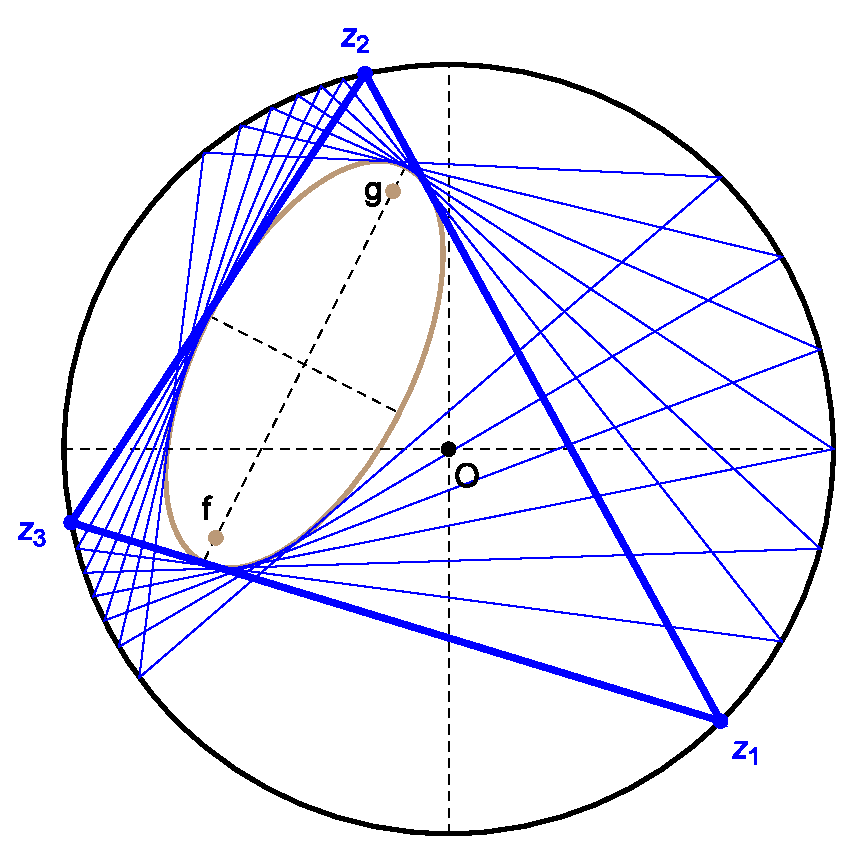
\includegraphics[width=.7\textwidth]{pics_04_050_blaschke_circum.eps}
    \caption{Blaschke complex parametrization of Poncelet 3-periodics (blue). Vertices are $z_1,z_2,z_3$. The foci of the caustic are $f,g$. }
    \label{fig:blaschke}
\end{figure}

%As a first step, identify points in $\R^2$ with points in the complex plane $\Cp$. Let $\D$ denote the open unit disk $\{z\in\Cp : |z|<1\}$ and $\T$ denote the unit circle $\{z\in\Cp : |z|=1\}$. By translation and scaling, we may assume the outer circle of the pair to be the unit circle $\T$. Let $\{f,g\}$ be the two foci of the inner ellipse.



Let  $\mathbb{T } = \{ z\in \mathbb{C}: |z| = 1\} $ the unit circle and $\mathbb{D} = \{ z\in\mathbb{C} : |z| < 1\} $ the open unit disk
bounded by $\mathbb{T }.$

Referring to \cref{fig:blaschke}, let $z_1,z_2,z_3\in\Cp$ denote the vertices of Poncelet 3-periodics in a generic $N=3$ family with fixed (unit) circumcircle denoted $\T=\{z\in\Cp : |z|=1\}$. Let $f,g$ be the foci of the caustic. Using Viète's formula, we obtain the following parametrization of the elementary symmetric polynomials on $z_1,z_2,z_3$ \cite{daepp-2019}:

\begin{definition}[Blaschke's Parametrization]
\begin{align*}
    \sigma_1:=z_1+z_2+z_3=& f+g+\l\ol f \ol g \\
    \sigma_2:=z_1 z_2+z_2 z_3+z_3 z_1=& f g+\l(\ol f+\ol g) \\
    \sigma_3:=z_1 z_2 z_3=& \l
\end{align*}
where $\l\in\T$ is the varying parameter.
\label{def:bla}
\end{definition}

\noindent Note that the concentric case occurs when $g=-f$.

For each $\l\in\T$, the three solutions of $B(z)=\l$ are the vertices of a 3-periodic orbit of the Poncelet family of triangles in the complex plane, \cite[Chapter 4]{daepp-2019}. Furthermore, as $\l$ varies in $\T$, the whole family of triangles is covered. Clearing the denominator in this equation and passing everything to the left-hand side, we get

\[
z^3-(f+g+\l\ol{f} \ol{g})z^2+(f g+\l(\ol f+\ol g))z-\l=0
\]

\begin{lemma}
If $u,v,w\in\mathbb{C}$ and $\lambda$ is a parameter that varies over the unit circle $\T\subset\mathbb{C}$, then the curve parametrized by
\[ F(\lambda)=u \lambda+ \frac{v}{\lambda}+w \]
is an ellipse centered at $w$, with semiaxis $|u|+|v|$ and $\big||u|-|v|\big|$, rotated with respect to the horizontal axis of $\mathbb{C}$ by an angle of $(\arg u+\arg v)/2$.
\label{lem:ell-param}
\end{lemma}

\begin{proof}
If either $u=0$ or $v=0$, the curve $h(\T)$ is clearly the translation of a multiple of the unit circle $\T$, and the result follows. Thus, we may assume $u\neq 0$ and $v\neq 0$.

Choose $k\in\mathbb{C}$ such that $k^2=u/v$. Write $k$ in polar form, as $k=r \mu$, where $r>0$ ($r\in\R$) and $|\mu|=1$. We define the following complex-valued functions:
\[R(z):=\mu z,~ S(z):=r z+(1/r) \ol{z},~ H(z):=k v z,~ T(z):=z+w\]

One can straight-forwardly check that $F=T\circ H\circ S\circ R$.

Since $|\mu|=1$, $R$ is a rotation of the plane, thus $R$ sends the unit circle $\T$ to itself. Since $r\in\R$, $r>0$, if we identify $\mathbb{C}$ with $\R^2$, $S$ can be seen as a linear transformation that sends $(x,y)\mapsto\left(\left(r+1/r\right)x,\left(r-1/r\right)y\right)$. Thus, $S$ sends $\T$ to an axis-aligned, origin-centered ellipse $\E_1$ with semiaxis $r+1/r$ and $|r-1/r|$. $H$ is the composition of a rotation and a homothety. $H$ sends the ellipse $\E_1$ to an origin-centered ellipse $\E_2$ rotated by an angle of $\arg(k v)=\arg(k)+\arg(v)=(\arg(u)-\arg(v))/2+\arg(v)=(\arg(u)+\arg(v))/2$. The semiaxis of $\E_2$ have length
\begin{align*}
|k v|&(r+1/r)=r|v|(r+1/r)=|r^2 v|+|v|=|k^2 v|+|v|=|u|+|v|\text{, and}\\
|k v|&|r-1/r|=r|v||r-1/r|=\big||r^2 v|-|v|\big|=\big||k^2 v|-|v|\big|=\big||u|-|v|\big|
\end{align*}

Finally, $T$ is a translation, thus $T$ sends $\E_2$ to an ellipse $\E_3$ centered at $w$, rotated by an angle $(\arg(u)+\arg(v))/2$ from the axis, with semiaxis lengths $|u|+|v|$ and $\big||u|-|v|\big|$, as desired.
\end{proof}

Consider the Moebius map $M_{z_0}=(z_0-z)/(1-\overline{z_0} z)$ and the Blaschke product of degree 3 given by   $B=M_{z_0} M_{z_1} M_{z_2}$.
\begin{theorem}
Let $B$ be a Blaschke product of degree 3 with
zeros $0, f, g.$ For $\lambda \in \mathbb{T}$, let $z_1, z_2, z_3 $ denote the three distinct solutions to $ B(z) = \lambda$. Then the
lines joining $z_j$ and $z_k$, $(j \ne k)$ are tangent to the ellipse given by
\[|w - f| + |w - g| = |1 -   \overline{f}   g |.\]
\end{theorem}
\begin{proof}
%\textcolor{red}{checar pagina}
See \cite[Theorem 2.9, page 37]{daepp-2019}.
\end{proof}

\begin{theorem}
 Given two points $f,g\in\mathbb{D}$. Then there exists a unique conic $\mathcal{E}$ with the foci
$f,g$   which is 3-Poncelet caustic with respect to $\mathbb{T}$. Moreover, $\mathcal{E}$ is an ellipse. That ellipse is
the Blaschke ellipse with the major axis of length $|1-\overline{f}g|.$
\end{theorem}

\begin{proof}
%\textcolor{red}{checar pagina}
See \cite[Corollary 4.4, page 44]{daepp-2019} and \cite{drag-milena2021}.
\end{proof}


 




\section{Locus of the Incenter in a CAP pair}
\label{sec:04-proof_theorem}
Recall the locus of the incenter (and excenters) are ellipses if the pair is confocal, see \cref{thm:03-incenter-excenter}. Here we expand the analysis and consider all CAP pairs.

\begin{proposition}\label{prop:04-X1c}
Over Poncelet 3-periodics in the pair with an outer circle and an ellipse in generic position, the locus $X_1$ is given by:
\begin{align*}
  X_1:&\;z^4 - 2(( \bar{f} + \bar{g}) \lambda +  f g) z^2 + 8   \lambda z\\
  &+ (\bar{f} - \bar{g})^2 \lambda^2 +2 (  |f|^2 g +   f |g|^2 - 2 f - 2 g) \lambda + f^2 g^2=0\\
  \;&:\;  z^4 - 2\beta  z^2+ 8\lambda z+  (\beta^2-4\alpha\lambda) =0
\end{align*}
\end{proposition}

\begin{proof} The incenter of a triangle with vertices $\{z_1,z_2,z_3\}$ is given by:
\begin{align*}
    X_1&=\frac{\sqrt{a}\;z_1+\sqrt{b}\;z_2+\sqrt{c}\;z_3}{\sqrt{a}+\sqrt{b}+\sqrt{c}}\\
    a&=|z_2-z_3|^2, \; b=|z_1-z_3|^2, \;\; c=|z_2-z_1|^2
\end{align*}
Using that $z_i\in \T$ it follows that
\[a=2-(\frac{z_3}{z_2}+\frac{z_3}{z_2}),\;\; b=2-(\frac{z_1}{z_3}+\frac{z_3}{z_1}),\;\;c=2-(\frac{z_1}{z_2}+\frac{z_2}{z_1})\]
Eliminating the square roots in  the equation $X_1-z=0$ and using the relations  $\sigma_i$ (i=1,2,3) given in Blaschke's parametrization the result follows.
\end{proof}

\begin{proposition}
\label{prop:04-X1g}
Over Poncelet 3-periodics in a generic nested ellipse pair, the locus of $X_1$ and the excenters is given by the roots of the following quartic polynomial in $z$:
{\small
\begin{align*}
X_1&: \;{\lambda}^{2} \left( p^2-q^2 \right) {
z}^{4}+4\,\lambda\, \left( \alpha\,\lambda\,p q^2  - q\,{
\lambda}^{2}p^{2}-\beta\,p^2\,q+p\,q^{2} \right) {z}^{3}\\
&+  ( 4\,\alpha\,{
\lambda}^{3}p^{3} q-4\,{\alpha}^{2}{\lambda}^{2}p^{2}q^2 +2\,\alpha\,\beta\,\lambda\,p^{3}
\,q-2\,\alpha\,\beta\,\lambda\,pq^{3} -2\,\beta\,{\lambda}^{2
}p^{4}+6\,\beta\,{\lambda}^{2}p^{2}q^2\\
&-6\,\alpha\,
\lambda\,p^2\,q^{2}+2\,\alpha\,\lambda\,q^{3} q+4\,{
\beta}^{2}p^2\,q^{2}  
  +6\,{\lambda}^{2}p^{3} \,q
 -6\,{
\lambda}^{2} p q^{3}  -4\,\beta\,p\,q^{3}  ) {z}^{
2}\\
&+ ( 4 q (\alpha^2\beta p^2 q^2 + 2\alpha^2 p^2  p q - \alpha^2 p q^3 + \beta^2 p^4 - 2\beta^2 p^2 q^2+ 4\beta p q^3 - p^2 q^2 - 2 q^4)\lambda \\
&- 4\alpha  p q^2 (\beta^2 p^2 - q^2) - 4 p^3 (\beta p  q - 2 p^2 - q^2)\lambda^3 - 16\alpha\lambda^2 p^4   q ) z\\
   & -\lambda^2 (4 \alpha \lambda - \beta^2) p^6 + 4 p^5 q \lambda^4 + 2 \lambda (4 \alpha^2 \lambda - \alpha \beta^2 - 3 \beta \lambda) p^5 q   - \lambda^2 (8 \alpha \lambda - 3 \beta^2) p^4 q^2 \\
   &+ (\alpha^2 \beta^2 -4 \alpha^3 \lambda  + 4 \alpha \beta \lambda + 5 \lambda^2) p^4 q^2 + 2 \lambda (2 \alpha^2 \lambda - \alpha \beta^2 + \beta \lambda) p^3 q^3 \\
   &+ (2 \alpha^2 \beta - 2 \alpha \lambda - 4 \beta^2) p^3 q^3 - (\alpha^2 \beta^2 + 4 \alpha \beta \lambda - 4 \beta^3 + 5 \lambda^2) p^2 q^4 + ( 8 \beta-3 \alpha^2 ) p^2 q^4 \\
   &+ (2 \alpha^2 \beta + 6 \alpha \lambda - 8 \beta^2) p q^5 - 4 q^5 p + ( 4 \beta-\alpha^2 ) q^6=0
\end{align*}
}
\end{proposition}

\begin{proof} Let $p,q\in \mathbb{R}$. Consider the affine transformation
$T(z)=pz+q\ol z$ and set $w_i=T(z_i)$. The proof is similar to that given in \cref{prop:04-X1c}. 
\end{proof}

\textcolor{red}{ronaldo: organiza, eu chamaria $p_1$ e $p_2$ talvez de $X_1$ e de $[e_1,e_2,e_3]$, mexer no exercicio.}

\begin{proposition} In the confocal pair the locus $X_1$ is defined by:


%\[2\,ab{\lambda}^{2}{z}^{2}+2\,\lambda\, \left( {a}^{3}{\lambda}^{2}-{b}
%^{3}{\lambda}^{2}-{a}^{3}-{b}^{3} \right) z+{c}^{2} \left( {c}^{2}{
%\lambda}^{4}-2\,ab{\lambda}^{2}-{c}^{2} \right)=0 \]
 \[   X_1 =z-\left({\frac { \left( a-b \right)  \left( -{a}^{2}-a b-{b}^{2}+\delta
 \right) \lambda}{2\,a b}}-{\frac { \left( a+b \right)  \left( -{a}^{2}
+a b-{b}^{2}+\delta \right) }{2\,a b\lambda}}\right)=0\]
\label{prop:04-X1q2} 
\end{proposition}

\begin{proof} In the confocal pair 
we have that
\[f={\frac {1}{c}\sqrt {-{a}^{2}-{b}^{2}+2\,\delta}}, \;\; g= -{\frac {1}{c}\sqrt {-{a}^{2}-{b}^{2}+2\,\delta}}\]
The result follows by factorization of the quartic  polynomial that defines $X_1$ in \cref{prop:04-X1c}.

Using CAS we obtain that $X_1$ is factorizable as $E_1 E_2$, where
\begin{align*}
    E_1&=z-\left({\frac { \left( a-b \right)  \left( -{a}^{2}-a b-{b}^{2}+\delta
 \right) \lambda}{2\,a b}}-{\frac { \left( a+b \right)  \left( -{a}^{2}
+a b-{b}^{2}+\delta \right) }{2\,a b\lambda}}\right)
\\
    E_2&=2 a b \lambda^2 z^3 - ((a - b) (a^2 + 3 a b + b^2 + \delta) \lambda^3 - (a + b) (a^2 - 3 a b + b^2 + \delta) \lambda) z^2\\
    &+ 6 a b  (a^2 - b^2) \lambda^2 z + (a + b)^3 (a^2 - a b + b^2 + \delta) \lambda^3 - (a - b)^3 (a^2 + a b + b^2 + \delta) \lambda
\end{align*}
\end{proof}

\begin{corollary}
The locus $X_1$ is the ellipse with semi-axes given by $a_1=(a^2-\delta)/b$ and $b_1=(\delta-b^2)/a.$

%\[z= {\frac { \left( a-b \right)  \left(\delta -{a}^{2}-ab-{b}^{2}
 %\right) \lambda}{2\,ab}}-{\frac { \left( a+b %\right)  \left(  \delta-{a}^{2}
%+ab-{b}^{2} \right) }{2\,ab\lambda}}\]
 
\end{corollary}

\begin{proof}
Follows directly from  \cref{lem:ell-param} and  \cref{prop:04-X1q2}.
\end{proof}

\begin{conjecture}
Over Poncelet 3-periodics in a given pair of conics, the locus of the incenter and excenters are ellipses if and only if the pair is confocal.
\label{conj:04-incenter-excenter-loci}
\end{conjecture}



\section{Loci in Generic Nested Ellipses}
\label{sec:04-loci}

 In this Section we prove the locus of a given fixed linear combination of $X_2$ and $X_3$ is an ellipse. We will use Blaschke products since, as shown in \cref{fig:04-affine}, a generic non-concentric pair is always the affine image of a pair with circumcircle.
 
 \begin{figure}
    \centering
    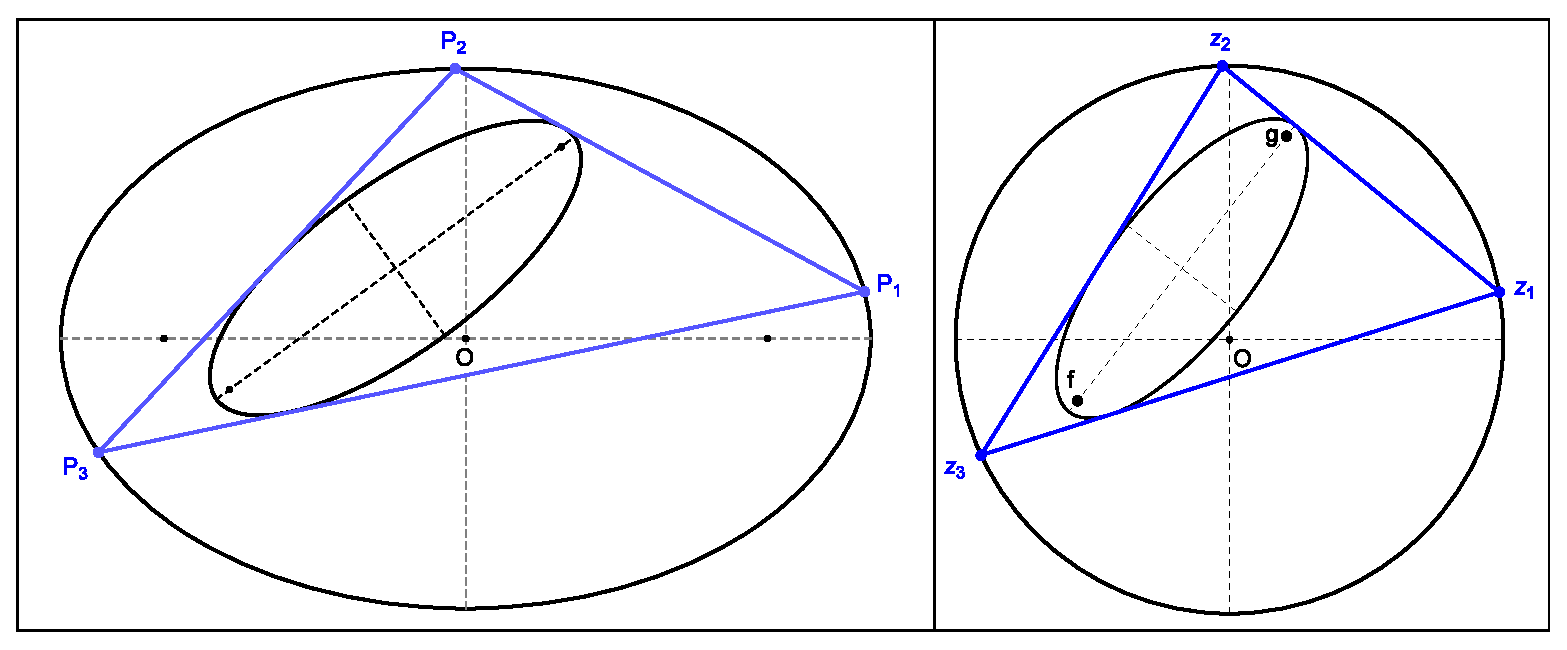
\includegraphics[width=\textwidth]{pics_04_030_affine_circumcircle.eps}
    \caption{Affine transformation that sends a generic ellipse pair and its 3-periodic family (left) to a new pair with circumcircle (right). We parametrize the 3-periodic orbit with vertices $z_i$ in the circumcircle pair using the foci of the latter's caustic $f$ and $g$, and then apply the inverse affine transformation to get a parametrization of the vertices $P_i$ of the original Poncelet pair. \href{https://youtu.be/6xSFBLWIkTM}{Video}}
    \label{fig:04-affine}
\end{figure}

\begin{figure}
    \centering
    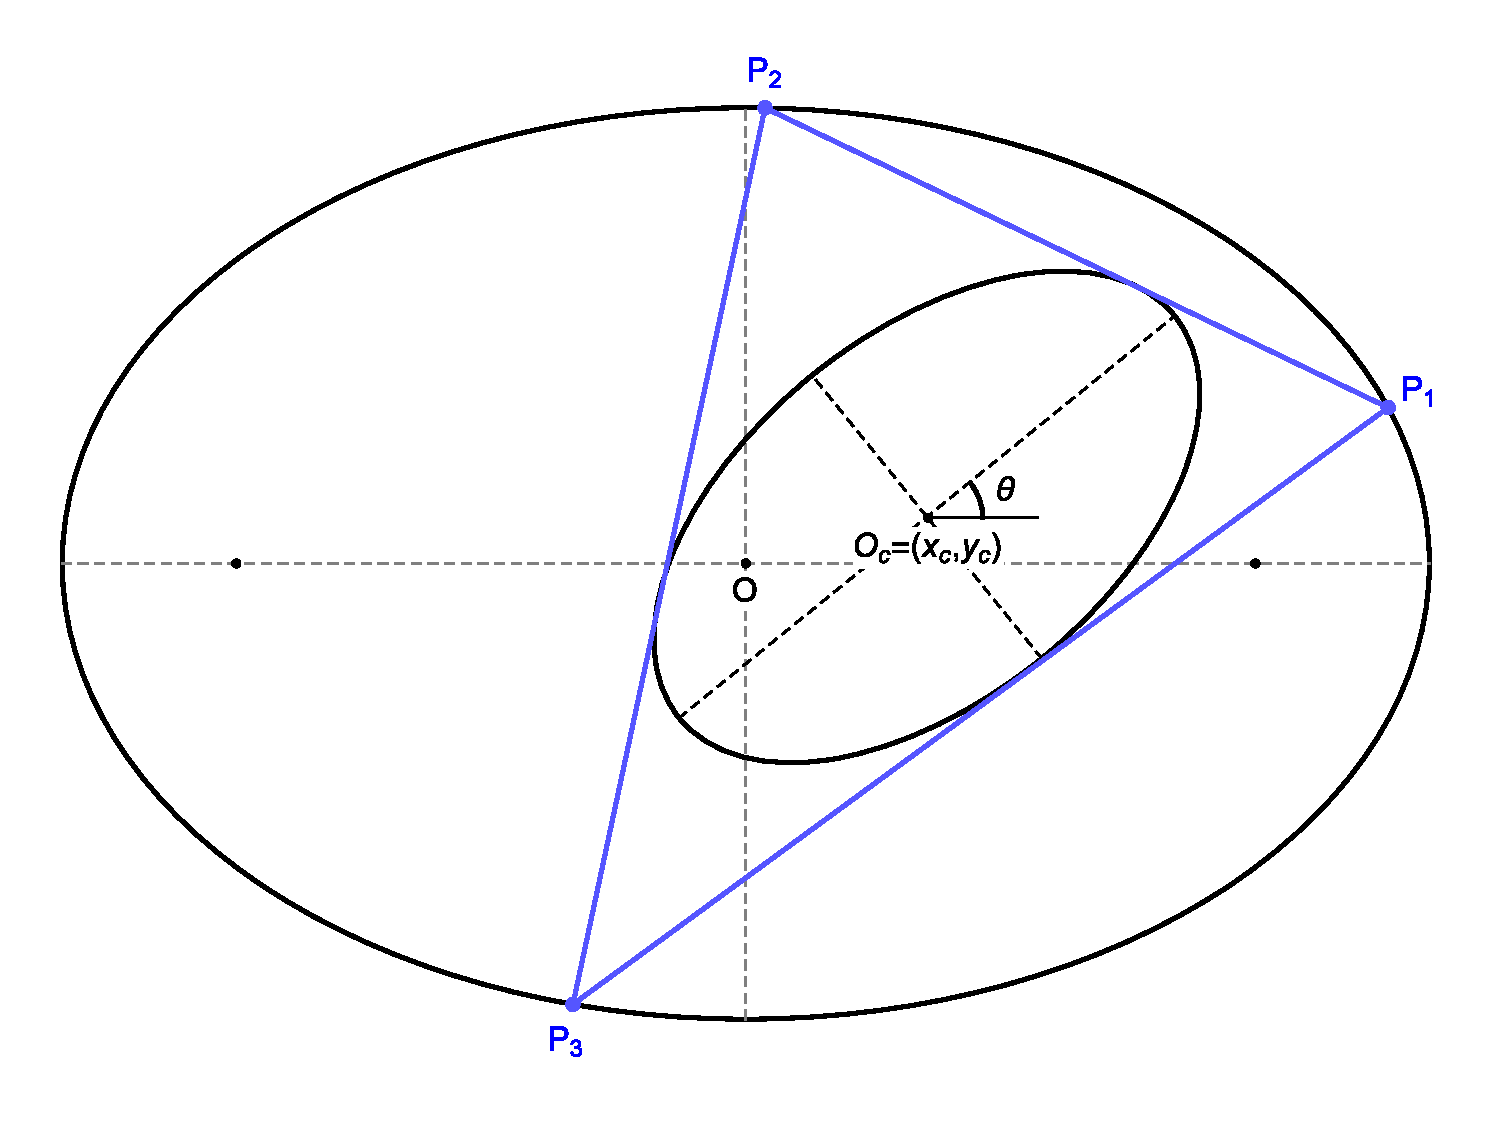
\includegraphics[width=.8\textwidth]{pics_04_010_n3_nonconcentric.eps}
    \caption{A pair of ellipses in general position which admits a Poncelet 3-periodic family (blue). Let the outer one be centered at the origin $O$. Their major axes are tilted by $\theta$, and their centers displaced by $O_c=(x_c,y_c)$. \href{https://youtu.be/bjHpXVyXXVc}{Video}}
    \label{fig:04-n3-nonconcentric}
\end{figure}

Consider the generic pair of nested ellipses $\E=(O,a,b)$ and $\E_c=(O_c,a_c,b_c.\theta)$ in Figure~\ref{fig:04-n3-nonconcentric}. Let s$\theta$, c$\theta$ denote the sine and cosine of $\theta$, respectively. Define $c_c^2=a_c^2-b_c^2$. The Cayley condition for the pair to admit a 3-periodic family is given by:

{\small
\begin{align}
&{b}^{4}x_c^{4}+2\,{a}^{2}{b}^{2}x_c^{2}y_c^{2}+
 \left(  2 c_c^2  \left( -{b}^{2}({a}^{2}+{b}^{2} )\right)  \text{c}\theta^2  - 2\left(  \,b ^{2}- \,b_c
^{2} \right) {b}^{2}{a}^{2}-2\,{b}^{4}b_c^{2} \right)x_c
^{2} \label{eqn:cayley}\\
&-8\,{a}^{2}{b}^{2}x_c\,{  y_c}\,c_c^2 
\text{s}\theta\text{c}\theta  +{a}^{4}y_c^{4} + \left(  2 c_c^2 a^2 \left(
{a}^{2}+{b}^{2}  \right)\text{c}\theta^2  
 -2 \left(  \,b_c^{2}+{b}^{2} \right) {a}^{4}+2
\,{a}^{2}{b}^{2}b_c^{2} \right) y_c^{2} \nonumber\\
&+ c_c^4  c^4  \left( \text{c}\theta^4-2\, c_c^2 c^2
  \left( {a}^{2} a_c^{2}-{b}^{2}{a}^{2}+
b_c^{2}{b}^{2} \right) \text{c}\theta^2 \right. \nonumber\\
 &+ \left( a a_c+a b-b b_c \right)  \left( a a_c
-a b -b b_c \right)  \left( a a_c+a b+b b_c \right)  \left( a
a_c-a b+b b_c \right) = 0\nonumber
\end{align}
}

%A related result is that the locus of the circumcenter-of-mass \cite{sergei2014-circumcenter-of-mass}, a generalization of $X_3$ for $N>3$ is also an ellipse.

Referring to Figure~\ref{fig:04-nonconcentric-xns}:

\begin{theorem}
Over the family of 3-periodics interscribed in an ellipse pair in general position (non-concentric, non-axis-aligned),
if $\X\ab$ is a fixed linear combination of $X_2$ and $X_3$, i.e., $\X\ab=\alpha X_2+\beta X_3$ for some fixed $\alpha,\beta\in\mathbb{C}$, then its locus is an ellipse. 
\label{thm:04-ellipse-locus}
\end{theorem}

\begin{proof}
Consider a general $N=3$ Poncelet pair of ellipses that forms a 1-parameter family of triangles. Without loss of generality, by translation and rotation, we may assume the outer ellipse is centered at the origin and axis-aligned with the plane $\R^2$, which we will also identify with the complex plane $\mathbb{C}$. Let $a,b$ be the semi-axis of the outer ellipse, and $a_c,b_c$ the semi-axis of the inner ellipse, as usual. 

Referring to Figure~\ref{fig:04-affine}, consider the linear transformation that takes $(x,y)\mapsto(x/a,y/b)$. This transformation takes the outer ellipse to the unit circle $\T$ and the inner ellipse to another ellipse. Thus, it transforms the general Poncelet $N=3$ system into a pair where the outer ellipse is the circumcircle, which we can parametrize using Blaschke products \cite{daepp-2019}. In fact, to get back to the original system, we must apply the inverse transformation that takes $(x,y)\mapsto(a x,b y)$. As a linear transformation from $\mathbb{C}$ to $\mathbb{C}$, we can write it as $L(z):=p z+q \ol{z}$, where $p:=(a+b)/2, q:=(a-b)/2$.

Let $z_1,z_2,z_3\in\T\subset\mathbb{C}$ be the three vertices of the circumcircle family, parametrized as in \cref{def:bla}, and let $v_1:=L(z_1),v_2:=L(z_2),v_3:=L(z_3)$ be the three vertices of the original general family. The barycenter $X_2$ of the original family is given by $(v_1+v_2+v_3)/3$, and the circumcenter $X_3$ is given by \cite{stackexchange-x3a}:

\[
    X_3=\left|
        \begin{array}{ccc}
          v_1 & |v_1|^2 & 1 \\
          v_2 & |v_2|^2 & 1 \\
          v_3 & |v_3|^2 & 1
        \end{array}
      \right| \Bigg/
     \left|
        \begin{array}{ccc}
          v_1 & \overline{v_1} & 1 \\
          v_2 & \overline{v_2} & 1 \\
          v_3 & \overline{v_3} & 1
        \end{array}
      \right|
\]

Since $\ol{z_1}=1/z_1,\ol{z_2}=1/z_2,\ol{z_3}=1/z_3$, we can write $v_1,v_2,v_3$ as rational functions of $z_1,z_2,z_3$, respectively. Thus, both $X_2$ and $X_3$ are symmetric rational functions on $z_1,z_2,z_3$. Defining $\X\ab=\alpha X_2+\beta X_3$, we have consequently that $\X\ab$ is also a symmetric rational function on $z_1,z_2,z_3$. Hence, we can reduce its numerator and denominator to functions on the elementary symmetric polynomials on $z_1,z_2,z_3$. This is exactly what we need in order to use the parametrization by Blaschke products.

In fact, we explicitly compute:
\[  \X\ab= \frac{p^2 q \left(\sigma_2 (\alpha +3 \beta )+3 \beta  \sigma_3^2\right)+\alpha  p^3 \sigma_1 \sigma_3-p q^2 (3 \beta +\sigma_1 \sigma_3 (\alpha +3 \beta ))-\alpha  q^3 \sigma_2}{3 \sigma_3 (p-q) (p+q)}\]
where $\sigma_1,\sigma_2,\sigma_3$ are the elementary symmetric polynomials on $z_1,z_2,z_3$.

Let $f,g\in\mathbb{C}$ be the foci of the inner ellipse in the circumcircle system. Using Definition~\ref{def:bla}, with the parameter $\l$ varying on the unit circle $\T$, we get:

\begin{equation}
\X\ab= u \l+v\frac{1}{\l}+w
\label{eqn:xi-param}
\end{equation}

\noindent where:

\begin{align*}
    u:=&\frac{p \left(\ol{f} \ol{g} \left(\alpha  p^2-q^2 (\alpha +3 \beta )\right)+3 \beta  p q\right)}{3 (p-q) (p+q)}\\
    v:=&\frac{\beta  p q (q-f g p)}{(q-p) (p+q)}+\frac{1}{3} \alpha  f g q\\
    w:=&\frac{q \left(\ol{f}+\ol{g}\right) \left(p^2 (\alpha +3 \beta )-\alpha  q^2\right)+p (f+g) \left(\alpha  p^2-q^2 (\alpha +3 \beta )\right)}{3 (p-q) (p+q)}
\end{align*}

By   \cref{lem:ell-param}, this is the parametrization of an ellipse centered at $w$, as desired. As in  \cref{lem:ell-param}, it is also possible to explicitly calculate its axis and rotation angle, but these expressions become very long.
\end{proof}

In \cref{thm:04-ellipse-locus} a linear combination of $X_2$ and $X_3$ was considered in terms of complex parameters $\alpha,\beta$. Below this result is specialized to the case of an affine combination of said centers in terms of a real parameter $\gamma$.

\begin{corollary}
Over the family of 3-periodics interscribed in an ellipse pair in general position (non-concentric, non-axis-aligned),
if $\X_\gamma$ is a real affine combination of $X_2$ and $X_3$, i.e., $\X_\gamma=(1-\gamma) X_2+\gamma X_3$ for some fixed $\gamma\in\R$, then its locus is an ellipse. Moreover, as we vary $\gamma$, the centers of the loci of the $\X_\gamma$ are collinear.
\end{corollary}

\begin{proof}
Apply   \cref{thm:04-ellipse-locus} with $\alpha=1-\gamma, \beta=\gamma$ to get the elliptical loci. As in the end of the proof of  \cref{thm:04-ellipse-locus}, the center of the locus of $\X_\gamma$ can be computed explicitly as 
\begin{gather*}
    w=w_0+w_1 \gamma \text{, where}\\
    w_0=\frac{1}{3} \left(q \left(\ol{f}+\ol{g}\right)+p (f+g)\right)\\
    w_1=\frac{q \left(2 p^2+q^2\right) \left(\ol{f}+\ol{g}\right)-p (f+g) \left(p^2+2 q^2\right)}{3 (p-q) (p+q)}
\end{gather*}
As $\gamma\in\R$ varies, it is clear the center $w$ sweeps a line.
\end{proof}

We proved that all of the following triangle centers have elliptic loci in the general N=3 Poncelet system, including the barycenter, circumcenter, orthocenter, nine-point center, and de Longchamps point (reflection of the orthocenter  about the circumcenter of a triangle):

\begin{observation}
Amongst the 40k+ centers listed on \cite{etc}, about 4.9k triangle centers lie on the Euler line \cite{etc-central-lines}. Out of these, only 226 are fixed affine combinations of $X_2$ and $X_3$. For $k<1000$, these amount to $X_k,k=${\small 2, 3, 4, 5, 20, 140, 376, 381, 382, 546, 547, 548, 549, 550, 631, 
632}.
\label{obs:affine-euler-line}
\end{observation}

\begin{figure}
     \centering
     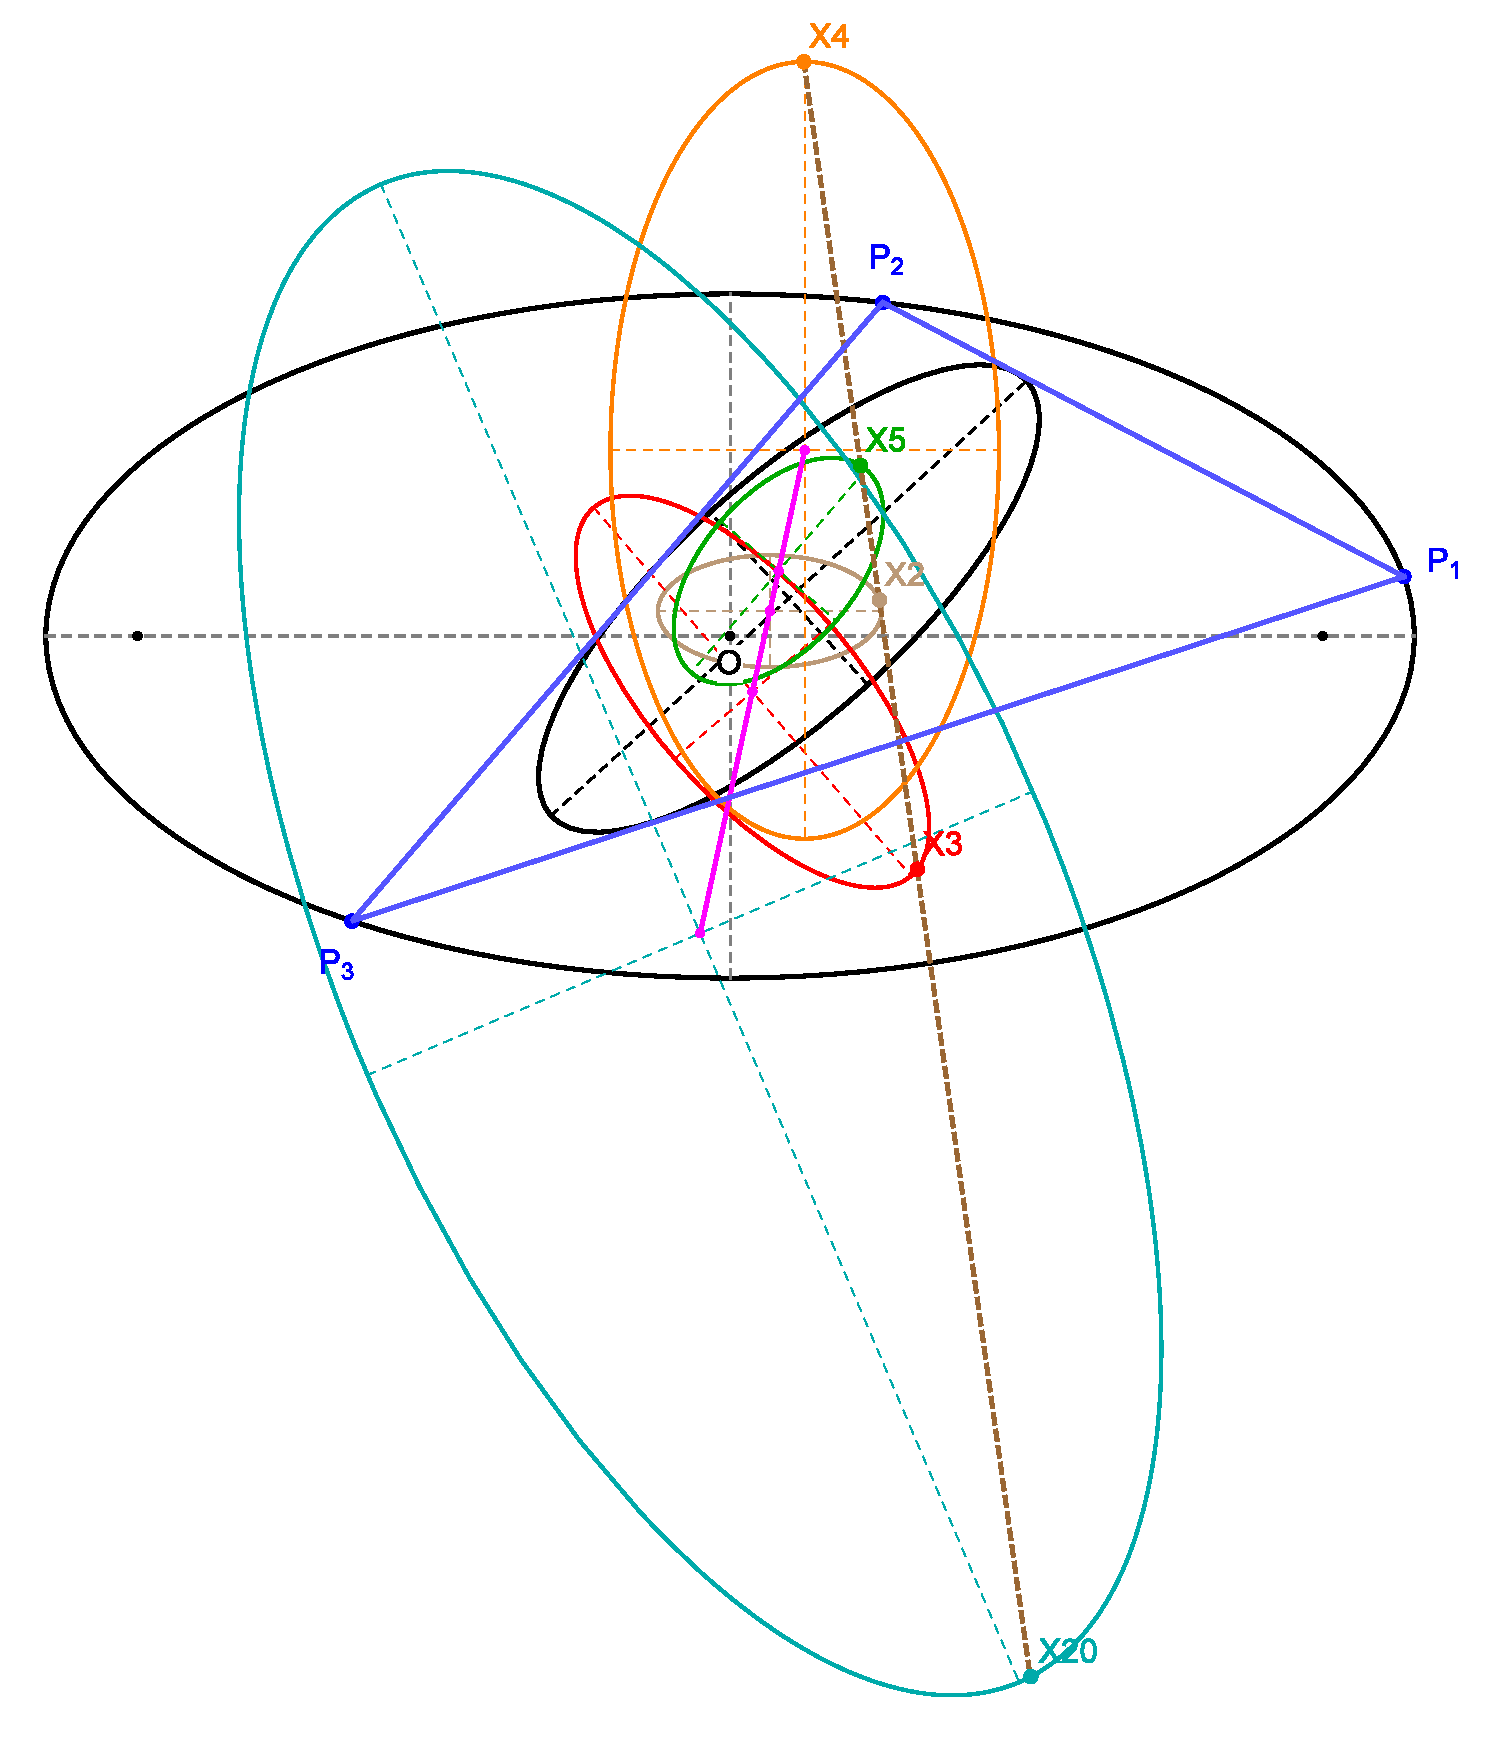
\includegraphics[width=\textwidth]{pics_04_020_n3_nonconcentric_loci.eps}
     \caption{A 3-periodic is shown interscribed between two nonconcentric, non-aligned ellipses (black). The loci of $X_k$, $k=2,3,4,5,20$ (and many others) remain ellipses. Those of $X_2$ and $X_4$ remain axis-aligned with the outer one. Furthermore the centers of all said elliptic loci are collinear (magenta line). \href{https://youtu.be/p1medAei_As}{Video}}
     \label{fig:04-nonconcentric-xns}
 \end{figure}
 
%\begin{corollary}
%The elliptic loci of $X_2$, $X_3$ and $X_4$ are given by:
%\[ \textcolor{red}{mark} \]
%\textcolor{red}{these will be hard to get explicitly}
%\end{corollary}
 
\begin{observation}\label{obs:X2X4}
The elliptic loci of $X_2$ and $X_4$ are axis-aligned with the outer ellipse.
\end{observation} 

%\begin{figure}
%    \centering
%    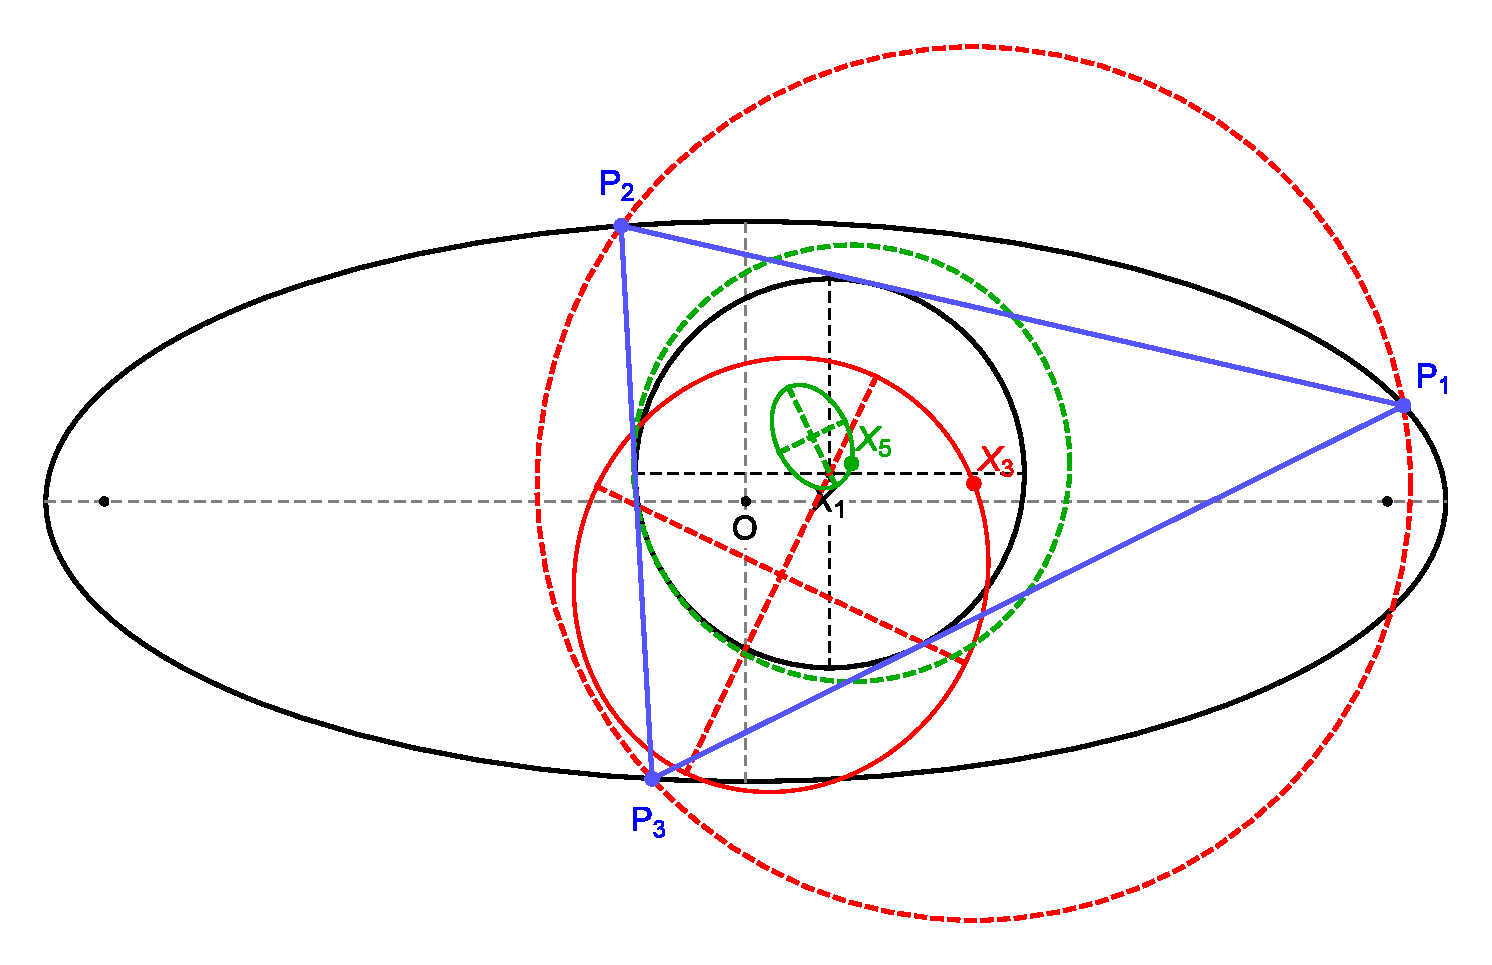
\includegraphics[width=.7\textwidth]{pics_04_040_n3_nonconcentric_circular_caustic.eps}
%    \caption{A 3-periodic (blue) is shown inscribed in an outer ellipse and an inner non-concentric circle centered on $O_c$. The loci of both circumcenter (solid red) and Euler center (solid green) are ellipses whose major axes pass through $O_c$. \href{https://youtu.be/w7sZ5O8k4xU}{Video}}
%    \label{fig:04-circular-caustic}
%\end{figure}

Experimental evidence suggests:

\begin{conjecture}
Over 3-periodics interscribed between two ellipses in general position, the locus of a triangle center $X_k$ is an ellipse if and only if $X_k$ is a fixed linear combination of $X_3$ and $X_4$.
\label{conj:04-locus}
\end{conjecture}



\section{Circular Loci in the Circumcircle Family}
\label{sec:04-circular}
\textcolor{red}{paper 11, family ties}

Referring to \cref{fig:04-nonconcentric-circular}:

\begin{proposition}
If a triangle center $\X\ab=\alpha X_2+ \beta X_3$ is a fixed linear combination of $X_2$ and $X_3$ for some $\alpha,\beta\in\mathbb{C}$, its locus over 3-periodics in the non-concentric pair with a circumcircle is a circle centered on $\mathcal{O}_\alpha$ and of radius $\mathcal{R}_\alpha$ given by:

\[ \mathcal{O}_\alpha = \frac{\alpha(f+g)}{3},\;\;\; \mathcal{R}_\alpha =\frac{|\alpha f g|}{3}\]
\label{prop:LinComb-concentric}

Furthermore, the center and radius of the locus do not depend on $\beta$ since the circumcenter $X_3$ is stationary at the origin of this system.
\end{proposition}

\begin{proof}
Since, $z_1,z_2,z_3$ are the 3 vertices of the Poncelet triangle inscribed in the unit circle, its barycenter and circumcenter are given by $X_2=(z_1+z_2+z_3)/3$ and $X_3=0$, respectively. We define $\X\ab:=\alpha X_2+ \beta X_3=\alpha (z_1+z_2+z_3)/3$. Using Definition~\ref{def:bla}, we get $\X\ab=\alpha(f+g+\l \ol{f}\ol{g})/3=\alpha(f+g)/3+\l(\alpha \ol{f}\ol{g})/3$, where the parameter $\l$ varies on the unit circle $\T$. Thus, the locus of $\X_{\gamma}$ over the Poncelet family of triangles is a circle with center $\mathcal{O}_{\alpha}:=\alpha(f+g)/3$ and radius $\mathcal{R}_{\alpha}:=|\alpha \ol{f}\ol{g}|/3=|\alpha f g|/3$.
\end{proof}

Using $\alpha=1-\gamma, \beta=\gamma$ for a fixed $\gamma\in\R$ in   \cref{prop:LinComb-concentric}, we get:

\begin{corollary}
 If a triangle center $\X_\gamma=(1-\gamma) X_2+ \gamma X_3$ is a real affine combination of $X_2$ and $X_3$ for some $\gamma\in\R$, its locus over 3-periodics in the non-concentric pair with a circumcircle is a circle. Moreover, as we vary $\gamma$, the centers of these loci are collinear with the fixed circumcenter.
 \label{cor:gamma-with-circumcircle}
\end{corollary}

Many triangle centers in \cite{etc} are affine combinations of the barycenter $X_2$ and circumcenter $X_3$. See   \cref{obs:affine-euler-line} for a compilation of them.

\begin{observation}
For a generic triangle, only $X_{98}$, and $X_{99}$ are simultaneously on the Euler line and on the circumcircle. However these are not linear combinations of $X_2$ and $X_3$. Still, if a triangle center is always on the circumcircle of a generic triangle (there are many of these, see \cite[Circumcircle]{mw}), its locus over 3-periodics in the non-concentric pair with circumcircle is trivially a circle.
\end{observation}

 
\begin{corollary}
 Over the family of 3-periodics inscribed in a circle and circumscribing a non-concentric inellipse centered at $O_c$, the locus of $X_k$, $k$ in 2,4,5,20 are circles whose centers are collinear. The locus of $X_5$ is centered on $O_c$. The centers and radii of these circular loci are given by:

\begin{alignat*}{4}
    O_2&=\frac{f+g}{3},\quad& O_4&=f+g,\quad&O_5&=\frac{f+g}{2},\quad&O_{20}&=-(f+g)\\
    r_2&=\frac{|f g|}{3},\quad&r_4 &= |f g|,\quad&r_5 &= \frac{|f g|}{2},\quad& r_{20}&= |f g|
\end{alignat*}

\end{corollary}

\begin{proof}
As in  \cref{cor:gamma-with-circumcircle}, we can use  \cref{prop:LinComb-concentric} with $\gamma=0,-2,-1/2,4$ to get the center and radius for $X_2,X_4,X_5,X_{20}$, respectively. All of these centers are real multiples of $f+g$, so they are all collinear. Moreover, the center $O_5$ of the circular loci of $X_5$ is $(f+g)/2$, that is, the midpoint of the foci of the inellipse, or in other words, the center $O_c$ of the inellipse.
\end{proof}
 
Referring to  \cref{fig:04-nonconcentric-circular}:

\begin{observation}
The family of 3-periodics in the pair with circumcircle includes obtuse triangles if and only if $X_3$ is exterior to the caustic. \end{observation}

This is due to the fact that when $X_3$ is interior to the caustic, said triangle center can never be exterior to the 3-periodic. Conversely, if $X_3$ is exterior, it must also be external to some 3-periodic, rendering the latter obtuse.

\begin{figure}
    \centering
    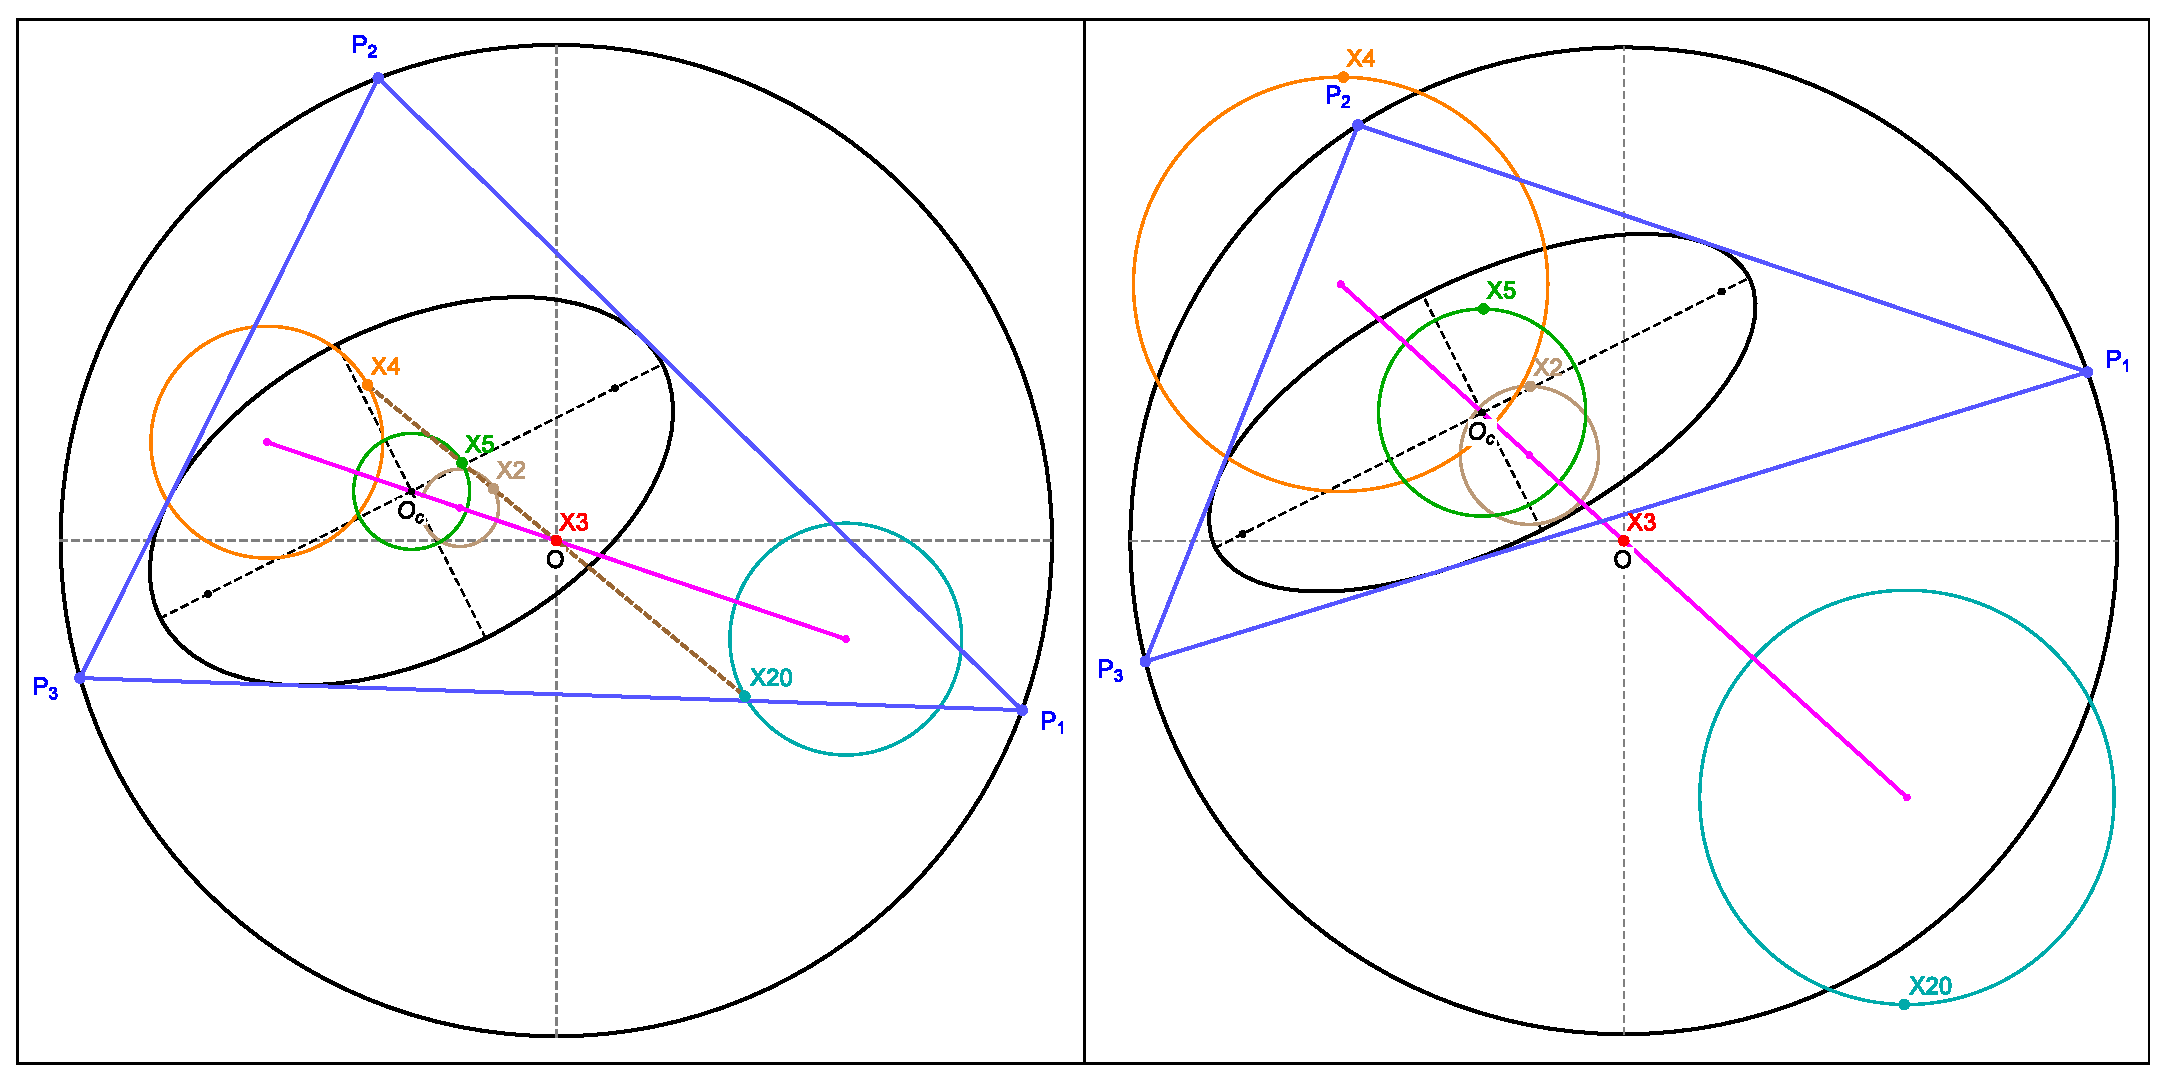
\includegraphics[width=\textwidth]{pics_03_010_n3_circumcircle_pair.eps}
    \caption{\textbf{Left:} 3-periodic family (blue) in the pair with circumcircle where the caustic contains $X_3$, i.e., all 3-periodics are acute. The loci of $X_4$ and $X_{20}$ are interior to the circumcircle. \textbf{Right:} $X_3$ is exterior to the caustic, and 3-periodics can be either acute or obtuse. Equivalently, the locus of $X_4$ intersects the circumcircle. In both cases (left and right), the loci of $X_k$, $k$ in 2,4,5,20 are circles with collinear centers (magenta line). The locus of $X_5$ is centered on $O_c$. The center of the $X_2$ locus is at $2/3$ along $O O_c$. \href{https://youtu.be/HXgJQo2UT_8}{Video}}
    \label{fig:04-nonconcentric-circular}
\end{figure} 






\section{Exercises}
\label{sec:04-exercises}
\section{Exercises}

\begin{exercise}
Show that over the poristic family, the locus of the foci of the $X_9$-centered circumconic (the circumbilliard) is a circle.
\end{exercise}

\begin{exercise}
Prove \cref{prop:04-antiorthic}. Furthermore, prove the intersection point of $X_1 X_3$ with the antiorthic axis is the Schröder point $X_{1155}$.
\end{exercise}

\begin{exercise}
Prove that over the poristic family the inconic centered on $X_1$ is axis-parallel with the circumconic centered on $X_9$ (i.e., the circumbilliard), see this \href{https://youtu.be/0VHBjdHXbJc}{Video}.
\end{exercise}


\begin{exercise}
Recall the cosine circle $\Cm$ (also known as the second Lemoine circle) is centered on a triangle's symmedian point $X_6$. Let $\E'$ be the Brocard ellipse of some triangle $T$. Let $\beta$ be the aspect ratio of $\E'$, i.e., $a'/b'$. Show that for any $T$, above (resp. below) a certain $\beta$, $\Cm$ is tangent to $\E'$ at two distinct points (resp. it is exterior to $\E'$). See it \href{https://bit.ly/2RqhUQV}{Live}.
\end{exercise}


\begin{exercise}
Show that the poristic excentral family is also the polar image of billiard excentrals wrt to a circle centered on a billiard (i.e., the caustic) focus. See it \href{https://bit.ly/33c1s9A}{Live}.
\end{exercise}

\begin{exercise}
Show that over the Brocard porism the radius $r^*$ of the cosine circle is invariant.
\end{exercise}

\begin{exercise}
Show that the first Lemoine circle (centered on $X_{182}$ is stationary over the Brocard porism. Above a certain $a'/b'$, this circle is tangent to one of the minor vertices of the caustic. See it \href{https://bit.ly/3tp0XUq}{Live}.
\end{exercise}

\begin{exercise}
Ehrmann's ``third'' Lemoine circle is studied in \cite{darij2012-ehrmann}, centered on $X_{576}$, is defined as follows: for each vertex, consider the 3 circles containing pairs of vertices and the symmedian point $X_6$. The third Lemoine circle contains the 6 intersections of said circles (2 each) with the sidelines. Prove this circle is also stationary over the Brocard porism, i.e., all three Lemoine circles are; see it \href{https://bit.ly/3tw09gA}{Live}. 
\end{exercise}


\begin{exercise}
Prove the expression and inequality for $\cot{\omega}$ in \cref{prop:04-brocard-w}.
\end{exercise}

\begin{exercise}
That the Brocard axis $X_3 X_6$ is stationary over the Brocard porism is established. Prove that the Lemoine axis, which intersects the Brocard axis at the Schoutte point $X_{187}$, is also stationary; see it \href{https://bit.ly/3nTRi75}{Live}.
\end{exercise}

\begin{exercise}
The so-called ``second'' Brocard triangle, defined in \cite[Second Brocard Triangle]{mw}, has vertices at the intersections of symmedians (cevians through $X_6$) with the Brocard circle. Show that over the Brocard porism, the family of second Brocard triangles is a new, smaller Brocard porism which shares the isodynamic points $X_{15}$ and $X_{16}$ with the original family. Prove that if this is iterated, the shrinking porisms converge to $X_{15}$. See it \href{https://bit.ly/3ttMNBg}{Live}.
\end{exercise}



\section{Research Questions}
\label{sec:04-research}
\section{Research Questions}

\begin{question}
Show that (i) the family of tangential triangles to the Brocard porism is also Ponceletian (caustic is the Brocard circumcircle).(ii) Derive the axes for the ellipse it is inscribed in.  and that (iii) its Gergonne point $X_7$ is stationary and coincides with the symmedian point $X_6$ of the Brocard porism; (iv) the locus of $X_{20}$ of the tangentials is a segment along the Brocard axis of the original family. \href{https://bit.ly/2RpNxdn}{Live} 
\end{question}

\begin{question}
The 3 Apollonius' circles of a triangle pass through a vertex and its two isodynamic points $X_{15}$ and $X_{16}$, see \cite[Isodynamic points]{mw}. Prove that over the Brocard porism, the sum of the inverse squared radii of the three Apollonius circles is invariant, see them \href{https://bit.ly/3elEzXI}{Live}.
\end{question}

\begin{question}
Prove that the polar image of the Brocard porism with respect to a circle centered on a caustic focus is another (tilted, smaller) Brocard porism whose Brocard inellipse shares a focus with the original one. Where does the sequence of Porisms converge? See it \href{https://bit.ly/3b7erOg}{Live}.
\end{question}

\begin{question}
Prove that over the poristic family, the barycenter $X_2$ of the intouch triangles is stationary. Derive its coordinates. See it \href{https://bit.ly/3i6DDsr}{Live}.
\end{question}
